\subsection{Mahalanobis distance}
\label{section:Mahalanobis}

\begin{figure}[t]
    \centering
    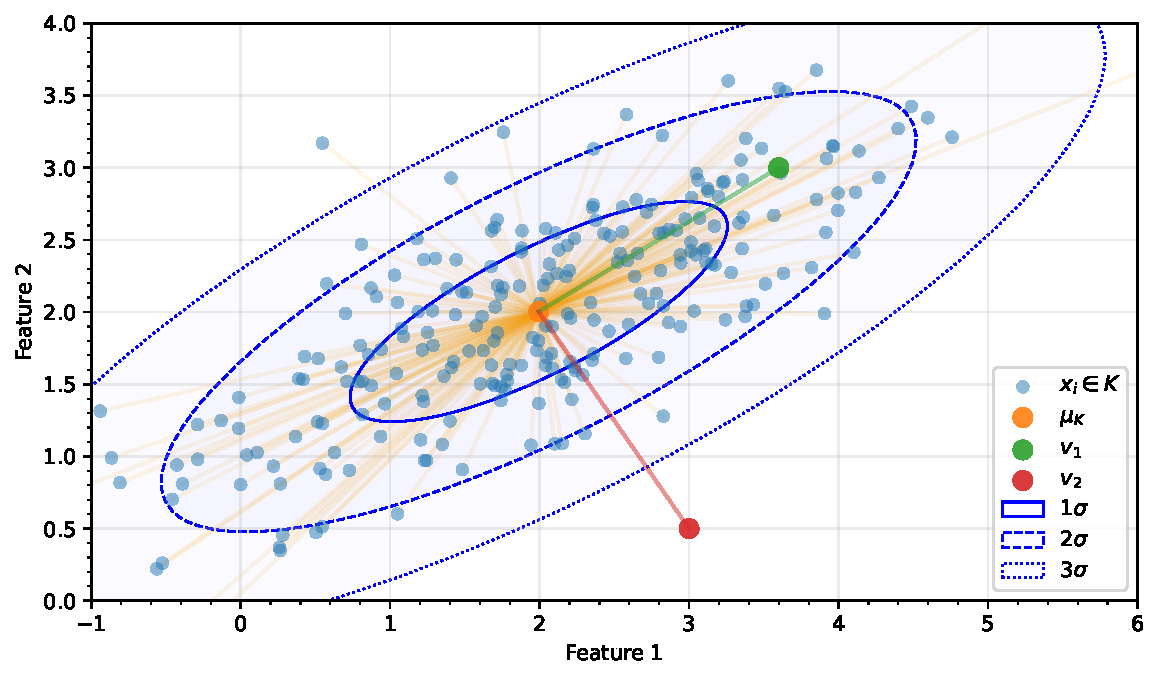
\includegraphics[width=\textwidth]{images/measures/mahalanobis-distance.pdf}
    \caption{Idea of the Mahalanobis distance applied as an outlierness measure.
             The~confidence ellipses indicate the distribution properties of cluster $T$;
             the marked areas correspond to regions in which about 68.2\%, 95.4\% and 99.7\%
             data are located. Despite that elements $v_1$ and $v_2$ have similar
             Euclidean distances from the cluster center $\mu_K$, only the element $v_1$
             is located in the more typical region, still surrounded by~elements $x_i \in T$,
             while $v_2$ shall be considered an outlier in this case.}
    \label{fig:md-idea}
\end{figure}

The Mahalanobis distance is one of the state-of-the-art solutions for performing out-of-distribution detection nowadays – often proposed directly as a method \cite{Lee-2018}\cite{Fort-2021}\cite{Du-2022}, mentioned in benchmarks \cite{Tajwar-2021}\cite{Zhou-2021}\cite{Podolskiy-2022}\cite{Yang-2022} or used as a baseline when compared with new techniques \cite{Liu-2020}\cite{Colombo-2022}\cite{Sun-2022}. It was originally described in 1936 by an Indian statistician P. C. Mahalanobis in \cite{Mahalanobis-1936} as a generalized distance metric for a~normally distributed multidimensional data, i.e., multivariate Gaussian distribution. It is claimed to be effectively applicable to high-dimensional data and promised to be more accurate than other measures, especially if there are correlated features in data.

It is an example of parametric method for outlier detection, that assumes in advance a specific characteristic of the data distribution, here: MVN (Multivariate Normal distribution); and the parameters of such a distribution, such as vector of means ($\mu$) and the covariance matrix ($\Sigma$), are estimated based on a provided training dataset.

The outlierness score for a given vector $v$ against the data cluster $T$ is calculated as
\begin{equation}
    MD(v, T) = \sqrt{
        (\vv{v - \mu_{T}})^{\top}
        \cdot
        \Sigma_{T}^{-1}
        \cdot
        (\vv{v - \mu_{T}})
    }.
    \label{eq:md}
\end{equation}

The $\mu_{T}$ represents the center of cluster $T$ – it is a vector of means of each variable ($\mu_{T} \in \mathbb{R}^d$). The $\Sigma_{T}^{-1}$ corresponds to the inverse of the covariance matrix $\Sigma_{T}$ calculated for the cluster $T$. In statistics the $\Sigma_{T}^{-1}$ element is also known as the precision matrix \cite{Wasserman-2010} (or concentration matrix).

High output values indicate the larger distance from the distribution center, suggesting that $v$ is potential outlier. Contrary, low values imply that $v$ resides close to the center of cluster $T$, conforming more to the data distribution and not being an outlier.

It shall be noticed that without the additional factor $\Sigma_{T}^{-1}$ the formula \ref{eq:md} would be an equivalent to the classical Euclidean distance in $\mathbb{R}^d$ space. Hence, the  $\Sigma_{T}^{-1}$ element can be interpreted as a scaling factor of the space where the distance is measured. In other words, the distance between analyzed point $v$ and the cluster center $\mu_{T}$ is adjusted to account the distribution shape, as the straight Euclidean distance along one axis can be more typical than the same straight distance along the axis where the data are more concentrated.

Figure \ref{fig:md-idea} illustrates such example, where the element $v_1$ can be considered as belonging to the data distribution, while the element $v_2$ is an outlier, despite the fact that both elements have similar Euclidean distance from the distribution center $\mu_{T}$.

It must be taken into account that as the estimation of the covariance matrix is required, fitting the algorithm to the training data can be computationally expensive if the datasets is large (i.e., big number of samples, high dimension of feature vectors). It is worth to notice that the typically used algorithms, like Maximum-Likelihood Estimation (MLE), are sensitive to the presence of any outliers in the dataset, so in cases where any contamination in the dataset may be present the literature suggests utilizing other techniques, such as the Minimum Covariance Determinant estimator \cite{Rousseeuw-1984}\cite{scikit-learn}\footnote{\scriptsize\url{https://scikit-learn.org/stable/auto_examples/covariance/plot_mahalanobis_distances.html}}.

Additional requirement for the inverse of covariance matrix $\Sigma^{-1}$ is that it must be positive-semidefinite and symmetric. The condition is that for a symmetric real matrix $M$ of dimension $d \times d$ there exist no such vector $v \in \mathbb{R}^d$ that would produce a negative result of a product $v^\top \cdot M \cdot v$; formally
\begin{equation}
    M = M^\top
    ~
    \land
    ~
    \forall v \in \mathbb{R}^d: v^\top \cdot M \cdot v \geq 0
    ~
    \Longleftrightarrow
    ~
    M ~ \text{is positive-semidefinite}.
    \label{eq:M-positive-semidefinite}
\end{equation}
When that condition is met, the $M$ can be expressed as a product of a lower triangular matrix $A$ and its transpose $A^\top$, i.e., $M = A^\top \cdot A$, known as the Cholesky decomposition \cite{Higham-1990}. Then, the product $v^\top \cdot M \cdot v$ is equal to the length of the vector $v$ transformed by the matrix $A$,
\begin{equation}
    v^\top \cdot M \cdot v
    =
    v^\top \cdot A^\top \cdot A \cdot v
    =
    (A \cdot v)^\top \cdot (A \cdot v)
    =
    \norm{A v}
    .
    \label{eq:M-length}
\end{equation}
Intuitively, this condition ensures that the output of formula \ref{eq:md} is not negative and can be interpreted as a distance metric. However, this condition cannot be satisfied when the number of samples $n$ is lower than features space dimension $d$ or the rank of the matrix $\Sigma^{-1}$ is lower than $d$ (as a result of highly correlated features or linearly dependent columns in the data – observed during research for ViT representation [section \ref{section:ViT}], further detailed study is needed).

Difficulties in practical applications for high-dimensional data involve the requirement of providing the sufficient number of training samples to fit the distribution model, i.e.~at~least $n_{T} \geq d$ and ideally $n_{T} \gg d$, for stable estimation of the covariance matrix $\Sigma_{T}$. However, for common datasets, such as \textit{ImageNet-1k} \cite{Russakovsky-2015}, there are underrepresented categories present that not satisfy this requirement, especially for large models with $d > 1000$ number of features, e.g., ResNet ($d = 2048$ features), ConvNeXT ($d = 1536$ features), EfficientNet ($d = 1280$ features). Hence, the approaches emerged, such as proposed in literature \cite{Lee-2018}\cite{Tajwar-2021}, to calculate the single covariance matrix $\Sigma$ using the whole training dataset for all classes as input, while still distinguishing means $\mu_{T}$ per data cluster during the distance calculation. This approach is sometimes called as utilizing the pooled covariance matrix \cite{Johnson-2007}\cite{Raninen-2022} and so the outlierness score can be calculated here for $m$ classes and vector of labels $y$ as follows:
\begin{equation}
    \Sigma
    =
    \frac{1}{n}
    \sum_{c=1}^{m}
    \sum_{i: y_i = c}^{n_c}
    (\vv{x_i - \mu_{c}})
    \cdot
    (\vv{x_i - \mu_{c}})^{\top}
    ,
    \label{eq:mdp-sigma}
\end{equation}
\begin{equation}
    MDP(v, T) = \sqrt{
        (\vv{v - \mu_{T}})^{\top}
        \cdot
        \Sigma^{-1}
        \cdot
        (\vv{v - \mu_{T}})
    }.
    \label{eq:mdp}
\end{equation}

During the research the implementation from the SciPy library \cite{SciPy-NMeth} was utilized.
